\subsubsection{Recurrent Networks}
\label{sec:theory-recurrent} 

Recurrent networks arise problems with computing their activations. For example imagine a cycle of neurons. That means that output of a particular unit could affect its input. Therefore the activations in general couldn't be computed only by one forward pass. This introduces real--valued dynamic systems for computing the activations. We can observe that it holds that $\frac{\partial\eta}{\partial t} = 0$ for the activations of neurons in the fixed point state. There are several approaches solving these dynamic systems and deriving the learning rule~\cite{pineda1987generalization, pearlmutter1989learning, williams1989learning, elman1990finding, haykin1994neural}. 

\begin{figure}[H]
  \centering
  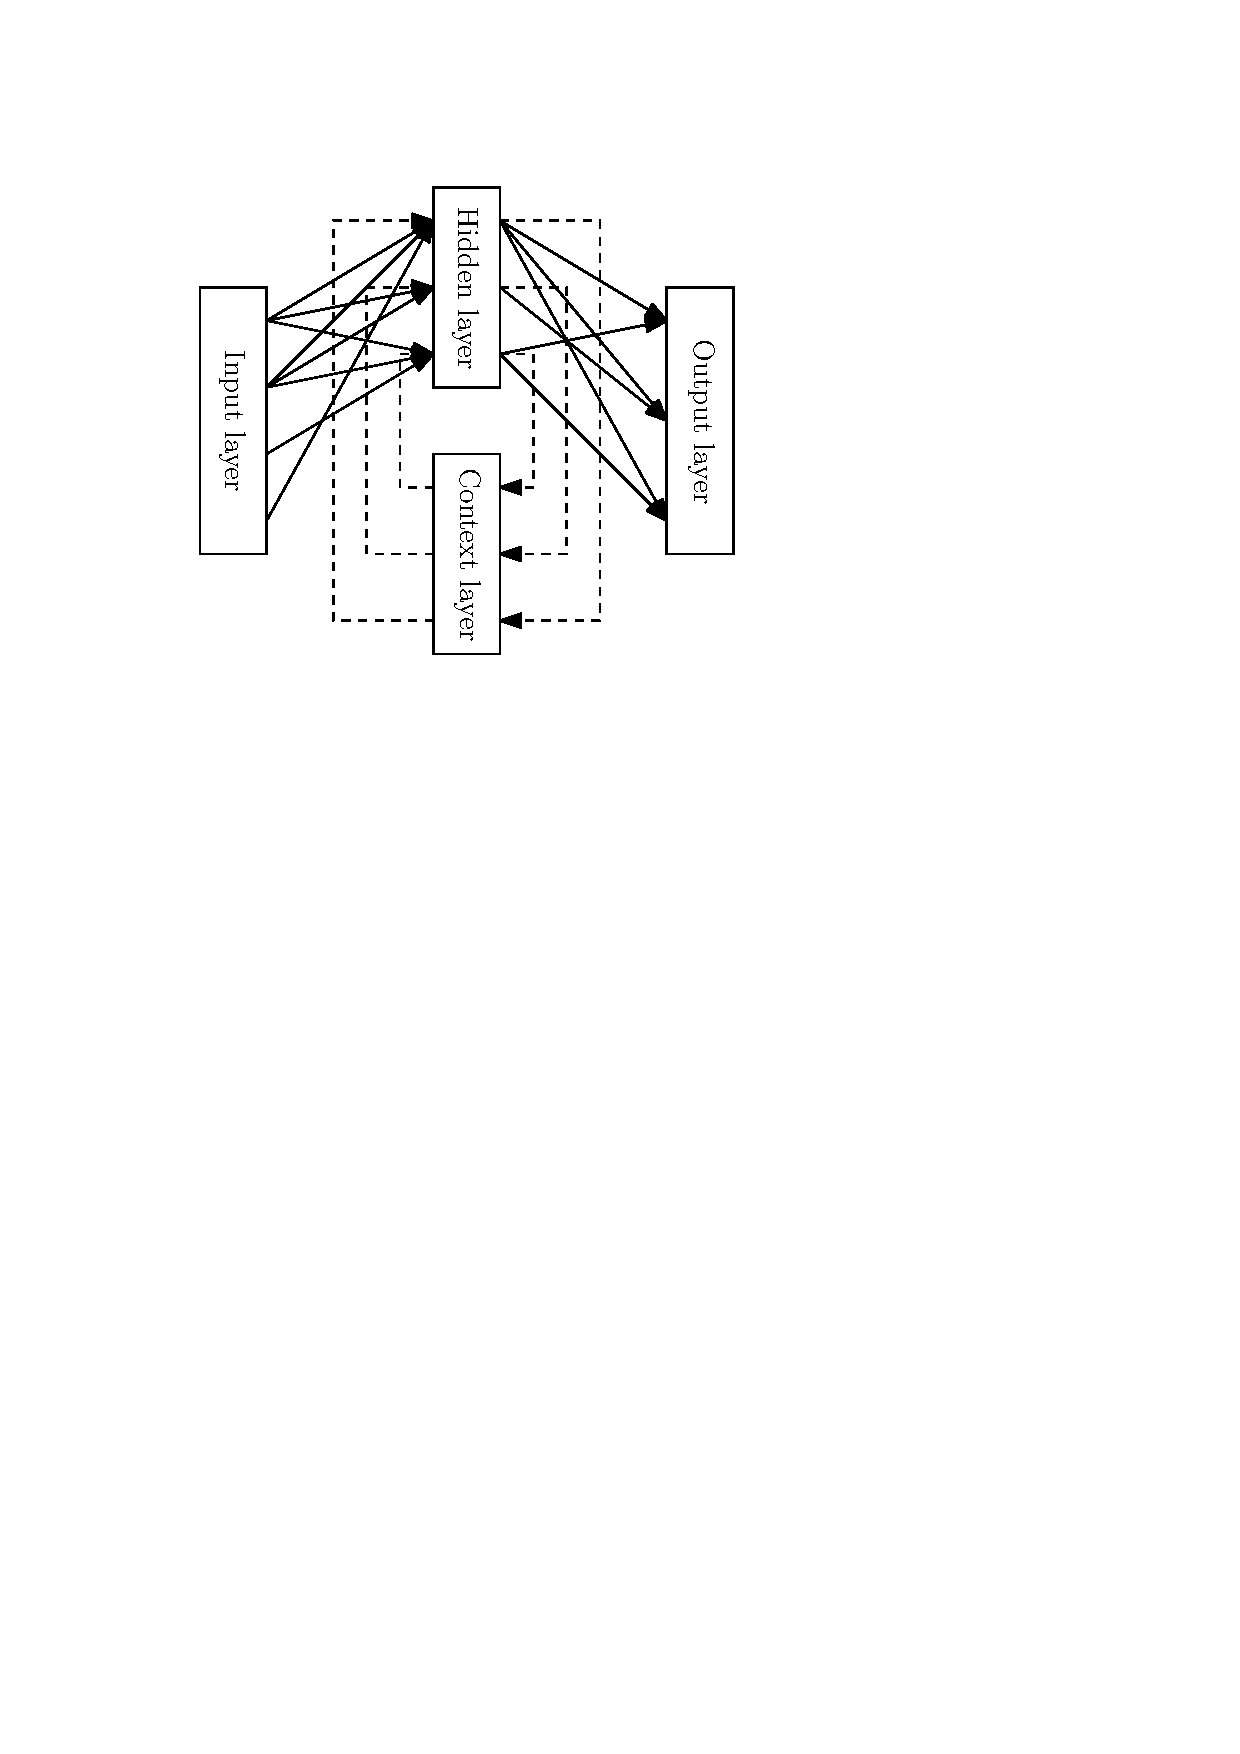
\includegraphics[width=0.4\textwidth]{img/models-recurrent.pdf}    
  \caption{Simple Recurrent network designed by~\citet{elman1990finding}. Image inspiration from~\citet{haykin1994neural}.} 
  \label{fig:theory-recurrent}
\end{figure}

An \emph{iterative method} is used by~\citet{movellan1990contrastive} for computing activations. In the first step the input neurons have activations equal to the input vector and the other neurons have zero activation. In the next steps activations from the last step are used to compute activation in this step as shown in equation~\ref{eq:theory-recurrent-activation}: 
\begin{equation}
  \label{eq:theory-recurrent-activation} 
  \eta_i(t+1) = \phi(\sum_j w_{ji}\eta_i(t)
\end{equation}
This rule is iterated while the activation are settled. For particullar symmetric network it could be proved that activations will converge~\citep{o1996bio}. For more general networks a dynamic system based on rule~\ref{eq:theory-recurrent-activation} could be derived and a fixed point solution could be found by solving a set of non--linear equations (TODO ref).~\citet{movellan1990contrastive} proposes using the method of simulated annealing~\citep{kirkpatrick1983optimization,vcerny1985thermodynamical} to improve the learning rule and to avoid settling the network in a local minima. We experimented with the iterative method for a two--way GeneRec~(\ref{sec:our-bal-recirc}). 

